%----------------------------------------------------------------------------
\label{iodine}
%----------------------------------------------------------------------------
Suppose the formalism from Section \ref{general dynamics} applies to the molecular iodine system and that there exists a transition in the dominant X-B system \cite{Tellinghuisen:1982a} for which the condition stated in Equation \ref{condition} can be met. The following equation relates $\bar{\mu}_e(R)$ (the electronic contribution to $M$ in the $R$ centroid approximation ) to $M_{ab}$ (from Equation \ref{matrix element}),
%----------------------------------------------------------------------------
\begin{equation}
\boxed{
M_{ab}
=
\bar{\mu}_e(R) \braket
{\nu^{\prime}}
{\nu^{\prime\prime}}
}
\end{equation}
%----------------------------------------------------------------------------
where $\bar{\mu}_e(R)$ is called the electronic transition moment and $\braket{\nu^{\prime}}{\nu^{\prime\prime}}$ is called the Franck--Condon factor (FCF) \cite{Koffend:1979a,Yazykova:1980a,Rapoport:1977a}.

Reference \cite{Lamrini:1993a} reports the squared \emph{electronic} dipole matrix element, $|\bar{\mu}_e(R_c)|^2=|\bar{\mu}_e|^2$, for molecular iodine to vary from a maximum of $(2.00\pm0.11)\mbox{ D}^2$ (or $\bar{\mu}_e \sim 4.7\cross10^{-28}$ Cm) to a minimum of $(8.7\pm4.6)\cross10^{-5}\mbox{ D}^2$ (or $\bar{\mu}_e \sim 5.7\cross10^{-30}$ Cm) for $R_c=2.66\mbox{ \AA}$ and $R_c=6.035\mbox{ \AA}$ respectively ($\mbox{D}=10^{-18}\mbox{ esu}$ and $1\mbox{ Cm}=2.99792458\cross10^{9}\mbox{ esu}$). Reference \cite{Tellinghuisen:1978a} calculates the FCFs for numerous transitions. Most seem to be between $10^{-2}$ and $10^{-3}$; thus, we assume that the transition under consideration here has a FCF in this range. Many transitions have small FCFs, for example for $\nu^{\prime}=\nu^{\prime\prime}=0$ the FCF is $1.429\cross10^{-9}$; however, the density of transitions in molecular iodine is high enough such that we can usually find a strong transition nearby -- even when dealing with a spectral window only a few hundred MHz wide. We will take the logarithmic average of $|M_{+}|=4.7\cross10^{-30}\mbox{ Cm}$ and $|M_{-}|=5.7\cross10^{-33}\mbox{ Cm}$ as an approximate coupling:
%----------------------------------------------------------------------------
\begin{equation}
M
\equiv
|M_{01}|
=
\exp{
\frac{\ln{|M_+|}+\ln{|M_-|}}{2}
}\mbox{ Cm}
\sim
1.6\cross10^{-31}\mbox{ Cm}.
\end{equation}
%----------------------------------------------------------------------------
 In Figure \ref{fluence} we plot Equation \ref{required fluence} (with $\Delta\cdot\tau=\pi/2$) for $M_+$, $M$, and $M_-$.
%----------------------------------------------------------------------------
%----------------------------------------------------------------------------
%----------------------------------------------------------------------------
%bb defines the bounding box for the pdf
%viewport defines the area of the pdf used
%in sidewaysfigure the last entry in bb moves the caption toward/away the pic
%in sidewaysfigure the second entry in bb moves the pic toward/away the caption
%----------------------------------------------------------------------------
\begin{figure}
\scalebox{0.8}[0.8]{
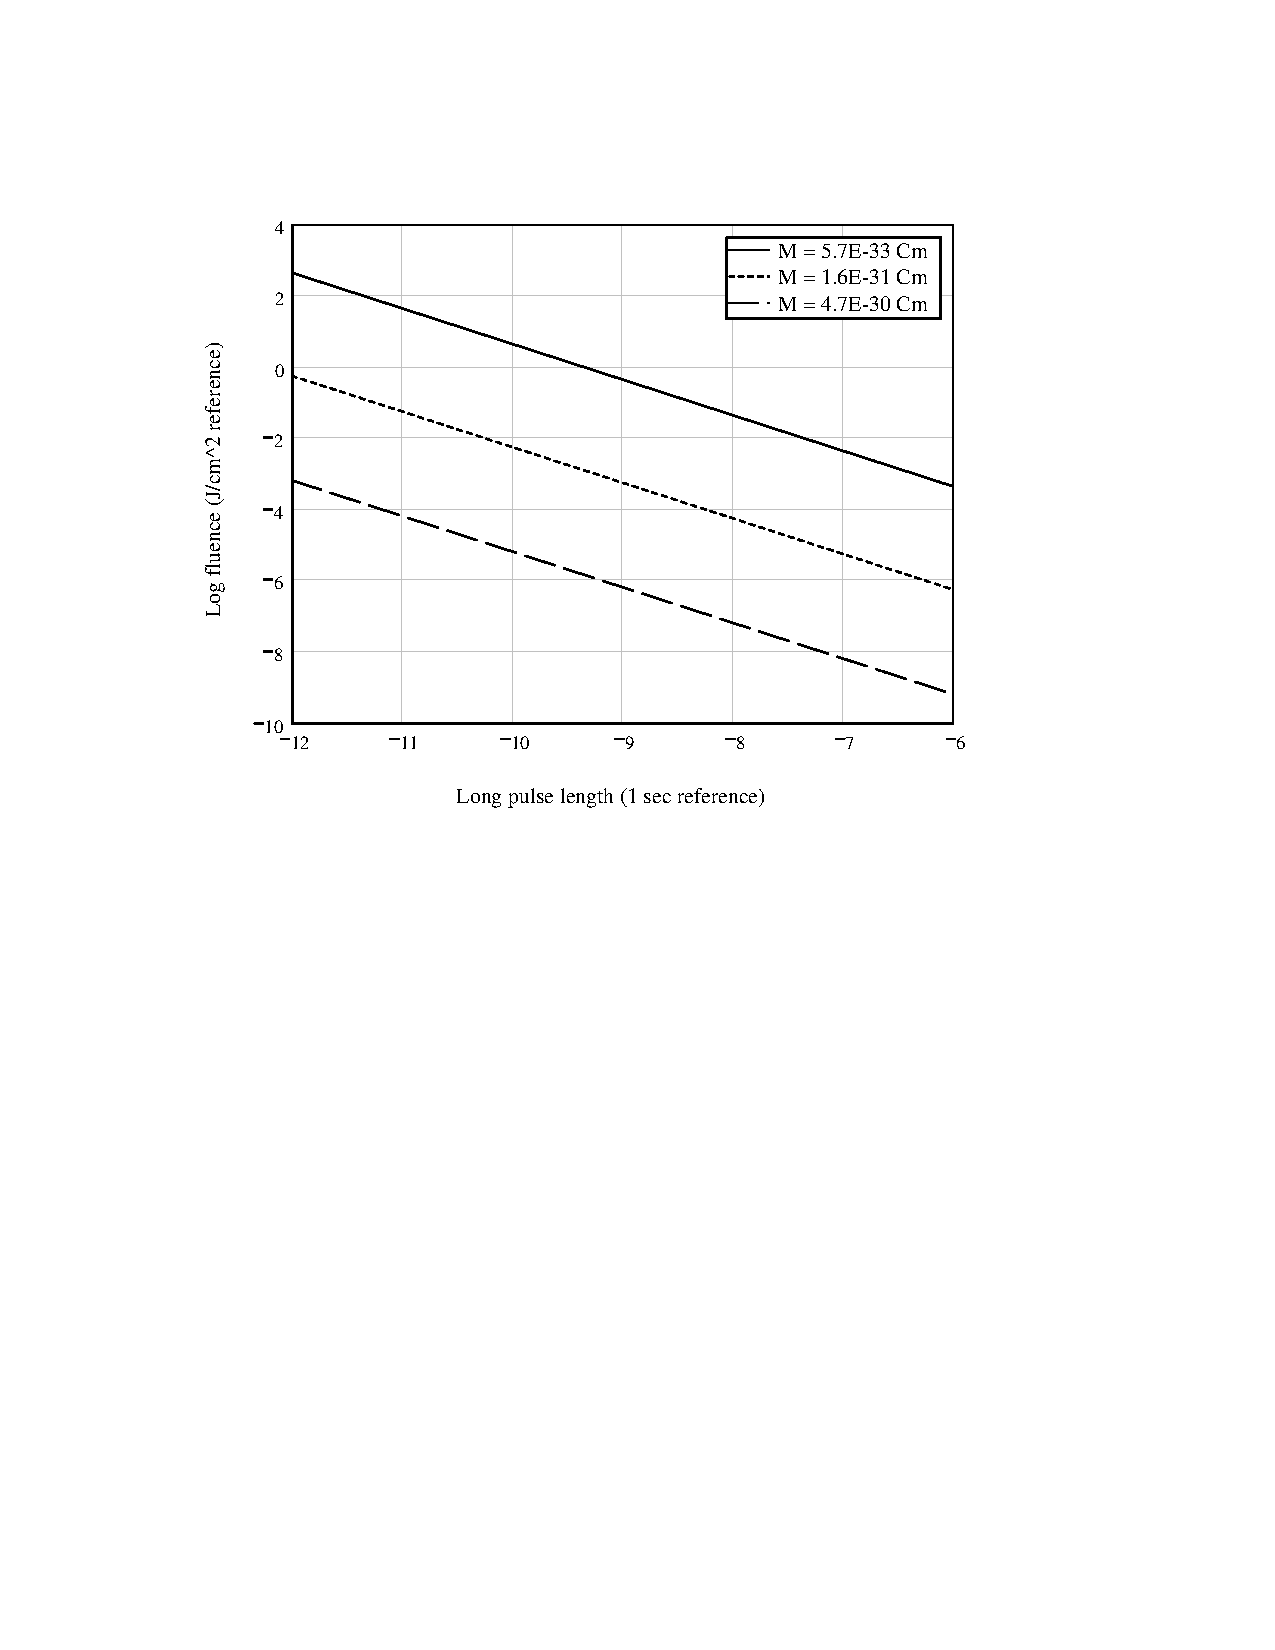
\includegraphics[bb=30 405 489 670]
{fluence/fluence.pdf}
}
\caption[Required fluence for inversion of the two level iodine molecule]{Required fluence for inversion of the two level iodine molecule. Here Equation \ref{required fluence} is plotted for various pulse lengths with $\Delta \tau = \pi/2$. To minimize the effect of collisions on the process, pulse length should be kept less that 1 ns when the target is at atmospheric pressure. A 1 ns pulse focused to a spot with a cross section area of about 1 mm$^2$ will need about 4 mJ to invert the two levels if we assume the ``weak'' coupling ($M=5.7\cross10^{-33}$ Cm). In an evacuated cell, one should be able to reduce the relaxiation effects to allow 100 ns pulses. In this case, the excitation beam (with the same 1 mm$^2$ cross section) must have over 0.7 mW of peak power, even when assuming ``strong'' coupling. ($M=4.7\cross10^{-30}$ Cm)}
\label{fluence}
\end{figure}
%----------------------------------------------------------------------------

%----------------------------------------------------------------------------
%----------------------------------------------------------------------------
%----------------------------------------------------------------------------
